% LTeX: language=es
% !TEX program = xelatex
% !TEX options = --shell-escape -synctex=1 -interaction=nonstopmode -file-line-error "%DOC%"

\documentclass[aspectratio=169]{beamer}

\usepackage[spanish,es-noshorthands]{babel}
\usepackage{color}
\usepackage{xcolor}

\usepackage{enumerate}
\usepackage{booktabs, multirow} % for borders and merged ranges
\usepackage{soul}% for underlines
\usepackage{changepage,threeparttable}
\usepackage{float}
\usepackage{listings}
\usepackage{pdfpages}
\usepackage{minted}
\usepackage{multicol}
\usepackage{filecontents}
\usepackage{url}

\usepackage{tikz}
\usetikzlibrary{shapes,arrows}

\newcount\mycount

%\graphicspath{{./}}

%\theoremstyle{definition}
%\newtheorem{definition}{Definici\'on}[section]
%\newtheorem{proposition}[definition]{Proposici\'on}
%\newtheorem{lemma}[definition]{Lema}
%\newtheorem{theorem}[definition]{Teorema}
%\newtheorem{corollary}[definition]{Corolario}
%\newtheorem{example}[definition]{Ejemplo}
%\newtheorem{observation}[definition]{Observaci\'on}
%\newtheorem{problem}{Problema}
%\newtheorem{question}[definition]{Pregunta}
\newtheorem{pointt}{}

\def\proof{\noindent{\textbf{Demostraci\'on}}\\}
\def\endproof{\hfill{\ensuremath\square}}
\def\refname{Referencias}
\allowdisplaybreaks



\usetheme{Boadilla}
\setbeamertemplate{blocks}[rounded][shadow=false]

\usefonttheme[onlymath]{serif}

\RequirePackage{fontspec}
%\setmainfont[Ligatures=TeX]{EB Garamond}
\setsansfont[Ligatures=TeX]{EBGaramond-VariableFont_wght.ttf}
%\setseriffont[Ligatures=TeX]{Raleway}
\newfontfamily\raleway{RalewayThin-wght350.ttf}
\newfontfamily\ebg{EBGaramond-VariableFont_wght.ttf}
%\newfontfamily{\semibold}{RalewayThin-Weight600}

\setmonofont{FiraCode-Regular.ttf}
%\usepackage{mathspec}
%\setmathrm{FiraCode-Regular.ttf}
%\setmathfont(Digits,Latin){FiraCode-Regular.ttf}
%\setmathfont[range=\mathit]{FiraCode-Regular.ttf}

\definecolor{backgroundColour}{RGB}{29, 29, 38}
\definecolor{textColour}{RGB}{179, 179, 212}
\definecolor{structureColour}{RGB}{255, 51, 153}
\definecolor{structure2Colour}{RGB}{204, 102, 255}
\definecolor{structure3Colour}{RGB}{255, 204, 102}
\setbeamercolor{normal text}{fg=textColour,bg=backgroundColour}
\setbeamercolor{structure}{fg=structureColour}

\setbeamercolor{palette primary}{use=structure,bg=structureColour, fg=textColour!50!white}
\setbeamercolor{palette secondary}{use=structure,bg=structureColour, fg=textColour!50!white}
\setbeamercolor{palette tertiary}{use=structure,bg=structureColour, fg=textColour!50!white}

\setbeamercolor{author}{fg=structure2Colour}
\setbeamercolor{subtitle}{fg=structure3Colour}
\setbeamercolor{alerted text}{fg=structure3Colour}
\setbeamercolor{highlighted}{fg=structure3Colour}

%\setbeamerfont{normal text}{family=\ebg}
%\setbeamerfont{structure}{family=\ebg}
%\setbeamerfont{block body}{family=\ebg}
\setbeamerfont{title}{size=\fontsize{18}{1},family=\raleway}
\setbeamerfont{frametitle}{size=\fontsize{18}{28},family=\raleway}



\title{Videojuegos e Inteligencia Artificial}

\author[Castro-Sotelo, García-Espinoza, Molina-Rebolledo] % (optional)
{C.A.~Castro-Sotelo \and A.T.~García-Espinoza \and I.~Molina-Rebolledo}

\institute[BUAP] % (optional)
{
  Facultad de Ciencias de la Computación\\
  Benemérita Universidad Autónoma de Puebla
}

\date[Otoño 2022] % (optional)
{Inteligencia Artificial, otoño 2022}



\date{14 de noviembre de 2022}
\def\code#1{\mintinline[fontsize=\small]{lean}{#1}}
%\beamerdefaultoverlayspecification{<+->}

\begin{document}
\frame{\titlepage}
%Highlighting text


\begin{frame}[fragile]
\frametitle{Videojuegos e Inteligencia Artificial}
\begin{columns}
\column{0.5\textwidth}
\begin{itemize}[<+->]
\item Cuando uno piensa en la inteligencia artificial en los videojuegos
  comúnmente se imagina la simulación de comportamientos de los personajes no
  manejados por el jugador.
\item La mayoría de videojuegos se trabajan con inteligencia artificial que
  permite que los personajes generados sean capaces de reaccionar según las
  circunstancias.
\end{itemize}
\column{0.5\textwidth}
\begin{center}
  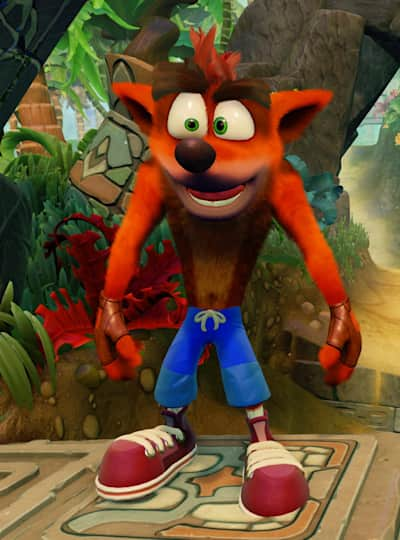
\includegraphics[width=0.4\textwidth]{./images/crash.jpg}
\end{center}
\end{columns}
\end{frame}

\begin{frame}
\frametitle{Videojuegos e Inteligencia Artificial}
\begin{columns}
\column{0.5\textwidth}
\begin{itemize}[<+->]
\item La inteligencia artificial también permite determinar el camino más corto
  que debe recorrer un personaje para ir entre el punto A y B, indica si está
  en peligro para huir o curarse aplicando algoritmos, entre otras
  aplicaciones.
\end{itemize}
\column{0.5\textwidth}
\begin{center}
  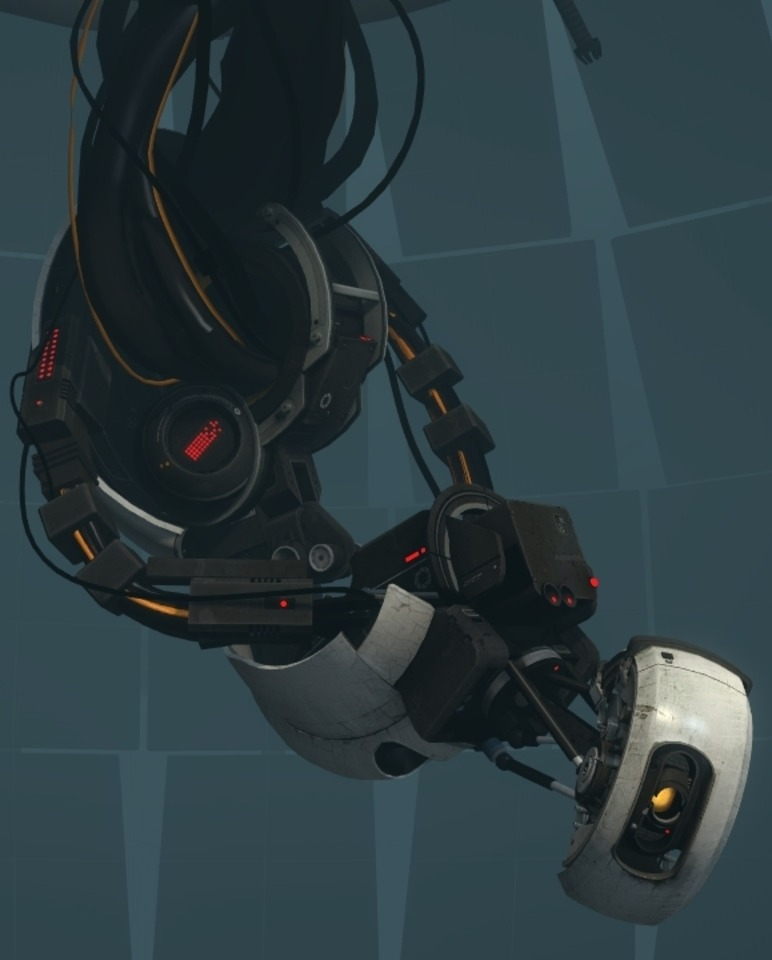
\includegraphics[width=0.4\textwidth]{./images/ai.jpeg}
\end{center}
\end{columns}
\end{frame}

\begin{frame}
\frametitle{Historia}
\begin{itemize}[<+->]
\item Fue los años 50 donde los primeros sistemas de inteligencia artificial se
  aplicaron a juegos de mesa: damas (Arthur Samuel) y ajedrez (Claude Shannon).
\item Para los años 60 se desarrollaron juegos como el Pong o Spacewar! basados
  en la lógica. 
\item En los 70 surgieron juegos de 1 jugador contra enemigos que se movían
  mediante patrones almacenados. 
\item En esta misma década, llegó Space Invaders (1978), el cual añadió
  dificultad creciente y respondía a las acciones del jugador.
\item En 1980, Pac-Man incorporó algoritmos de búsqueda en laberintos. 
\item Llegando a los años 90, surgió Dragon Warrior, el primer RPG que permitía
  variar las rutinas de la IA de los enemigos durante las batallas.
\item Fue en esta década que se produjo un boom de nuevos géneros y nuevas
técnicas de IA: máquinas de estados finitos, redes neuronales, computación
evolutiva, lógica difusa, etc. Aquí tenemos a Battlecruiser 3000AD (1996)
que incorpora redes neuronales.
\end{itemize}
\end{frame}

\begin{frame}
\begin{center}
La meta de la investigación en inteligencia artificial es inventar una
verdadera inteligencia artificial. En orden para construir una inteligencia
artificial completa necesitamos construir un sistema que tome acciones en un
tipo de ambiente.
\end{center}
\end{frame}

\begin{frame}
\begin{center}
Video.
\url{https://www.youtube.com/watch?v=Elwb2lV88hM}
\end{center}
\end{frame}

\begin{frame}
\frametitle{En la práctica...}
\begin{itemize}[<+->]
\item Una de las ideas más obvias para llevar esto a cabo sería incorporar una
  inteligencia artificial en robots.
\item La práctica, sin embargo, nos ha mostrado que incluso las tareas más
  mundanas son difíciles de realizar por robots. 
\item Trabajar con robots claramente tiene sus desventajas: son caros y lentos.
\item Un robot requeriría de mucho tiempo de entrenamiento y el desarrollo de
  pistas que prueben y desafíen el sistema en su toma de decisiones.
\end{itemize}
\end{frame}

\begin{frame}
\begin{center}
Es por esto que tomaremos la perspectiva de los videojuegos como pruebas de
rendimiento para las inteligencias artificiales.
\end{center}
\end{frame}

\begin{frame}
\begin{itemize}[<+->]
\item Alan Turing, (re)inventó el algoritmo Minimax y lo usó para jugar ajedrez.
\item Arthur Samuel usó el aprendizaje por refuerzo en un programa que aprendió a jugar
damas jugando contra sí mismo.
\item Deep Blue de IBM ganó contra el famoso Gary Kasparov, en un evento en
1997; y AlphaGo, un programa para jugar Go de Google, logró vencer al
campeón europeo de este juego.
\end{itemize}
\end{frame}


\begin{frame}
\frametitle{Importancia}
\begin{itemize}[<+->]
\item Los videojuegos involucran múltiples sentidos y múltiples habilidades cognitivas.
\item Se ejecutan dentro de ellos ambientes controlables.
\item Estas características vuelven a los videojuegos buenas pruebas de rendimiento para
  las inteligencias artificiales.
\end{itemize}
\end{frame}

\begin{frame}
\frametitle{El estado actual}
\begin{itemize}[<+->]
\item Se han organizado competiciones donde los investigadores presentan sus
  inteligencias artificiales.
\item Tener competiciones recurrentes basadas en el mismo juego permite a los
  competidores refinar sus enfoques y métodos.
\item Los juegos más populares para estas competiciones son: Super Mario Bros,
  StarCraft, el juego de carreras TORCS,  Ms. Pac-Man, juegos genéricos del estilo
  de combate de Street Fighter, Angry-Birds, etc.
\item Estas competiciones juegan un papel importante en catalizar la investigación;
  cada año varios artículos científicos son publicados sobre los resultados.
\end{itemize}
\end{frame}

\begin{frame}
\frametitle{El estado actual II}
\begin{itemize}[<+->]
\item La especificidad del juego genera un gran problema.
\item Lo mejor que se puede hacer es probarlas en un número de problemas
  desconocidos.
\item El diseñador de la inteligencia artificial no debe conocer en qué
  problemas será probado su IA.
\end{itemize}
\end{frame}

\begin{frame}
\frametitle{El estado actual III}
\begin{itemize}[<+->]
\item Hay competiciones que permiten a sus concursantes enviar sus mejores inteligencias artificiales
  para que sean probadas en un juego a ciegas.
\item generar nuevos videojuegos para probar las inteligencias artificiales no
  es una tarea fácil.
\item Cameron Browne ya ha construido un generador completo para juegos de mesa
  jugables, y varias personas ya han intentado automatizar la generación de
  videojuegos.
\item Este mismo software podría ser usado fuera de las competiciones.
\end{itemize}
\end{frame}

\begin{frame}
\frametitle{En un futuro...}
\begin{itemize}[<+->]
\item Se espera tener algún software que permita la generación de videojuegos
  que nadie ha visto anteriormente.
\item Esto permitiría a los investigadores probar sus inteligencias artificiales
  en un número infinito de juegos.
\item En cuanto a la inteligencia artificial dentro de los videojuegos, se nos
  pinta una idea aún más grande.
\item Podríamos conseguir mismo videojuego se adapte al estilo del jugador,
  darle más acción al jugador si así lo prefiere o darle más historia si se adapta
  más al gusto del jugador
\end{itemize}
\end{frame}


% End of document
\begin{frame}
\frametitle{Final de la presentación}

Muchas gracias por su atención.
\end{frame}

\begin{frame}
\frametitle{Referencias}
\begin{itemize}
\item Alcalá, J. (n.d.). Inteligencia Artificial en Videojuegos [Slideshow]. 
\url{http://www.flasentertainment.com/blog/ia.pdf}
\item Togelius, J. (2017). AI Researchers, Video Games Are Your Friends!. In: , et al. 
Computational Intelligence. IJCCI 2015. Studies in Computational Intelligence, vol 669. 
Springer, Cham. \url{https://doi.org/10.1007/978-3-319-48506-5\_1} 
\item Rozo, E. J. B., Montoya, R. C., \& Páez, J. (2018). Videojuegos: Avances tecnológicos en 
aplicación de física e inteligencia artificial. Letras ConCiencia TecnoLógica, 61-78.
\item Perez-Liebana, D., Samothrakis, S., Togelius, J., Schaul, T., \& Lucas, S. M. 
(2016, March). General video game ai: Competition, challenges and opportunities. 
In Thirtieth AAAI conference on artificial intelligence.
\end{itemize}
\end{frame}

\begin{frame}
\frametitle{Ejercicio}

\begin{center}
Vamos a realizar un ejercicio para que vean la importancia de la inteligencia
artificial en los videojuegos.
\end{center}
\end{frame}

\end{document}
